\section{Implementation}
\label{sec:impl}

To evaluate in-network obfuscation on production-representative hardware, we implemented the defense
as a single P4$_{16}$ program for one Intel Tofino-1 switch, together with a control-plane
configuration layer and a guarded control-test harness. The data plane comprises six major parts:
(i)~a parser and transaction classifier; (ii)~an absolute-timestamp deadline stage; (iii)~a packet
generator that seeds strict-priority blocker reservoirs; (iv)~the response-shaping release, replication, and
egress carving path; (v)~the control-command epoch-and-hold state machine; and (vi)~two independent
Traffic-Manager scheduling domains. A single terminal table applies every port, queue, drop, bypass,
and multicast effect. The program fits in one ingress pipe within the twelve-stage match-action
budget.

\subsection{Physical topology and port roles}
The master, the switch, and the outstation sit in one line: the master reaches the switch on device
port \code{dp9}, and the switch reaches the physical SEL-751 on \code{dp64}. Three ports are internal
to the switch and carry no external cable: \code{dp8} recirculates responses for the response-shaping ladder,
\code{dp10} holds the OPERATE for the control-command hold, and \code{dp68} injects generated tokens and clones. The
adversary's observation point is the master-facing link at \code{dp9}; the relay-facing link at
\code{dp64} and the internal ports are not part of the observed traffic. We treat \code{dp8},
\code{dp10}, and \code{dp68} as switch implementation details, not additional inline devices.

\begin{figure*}[t]
\centering
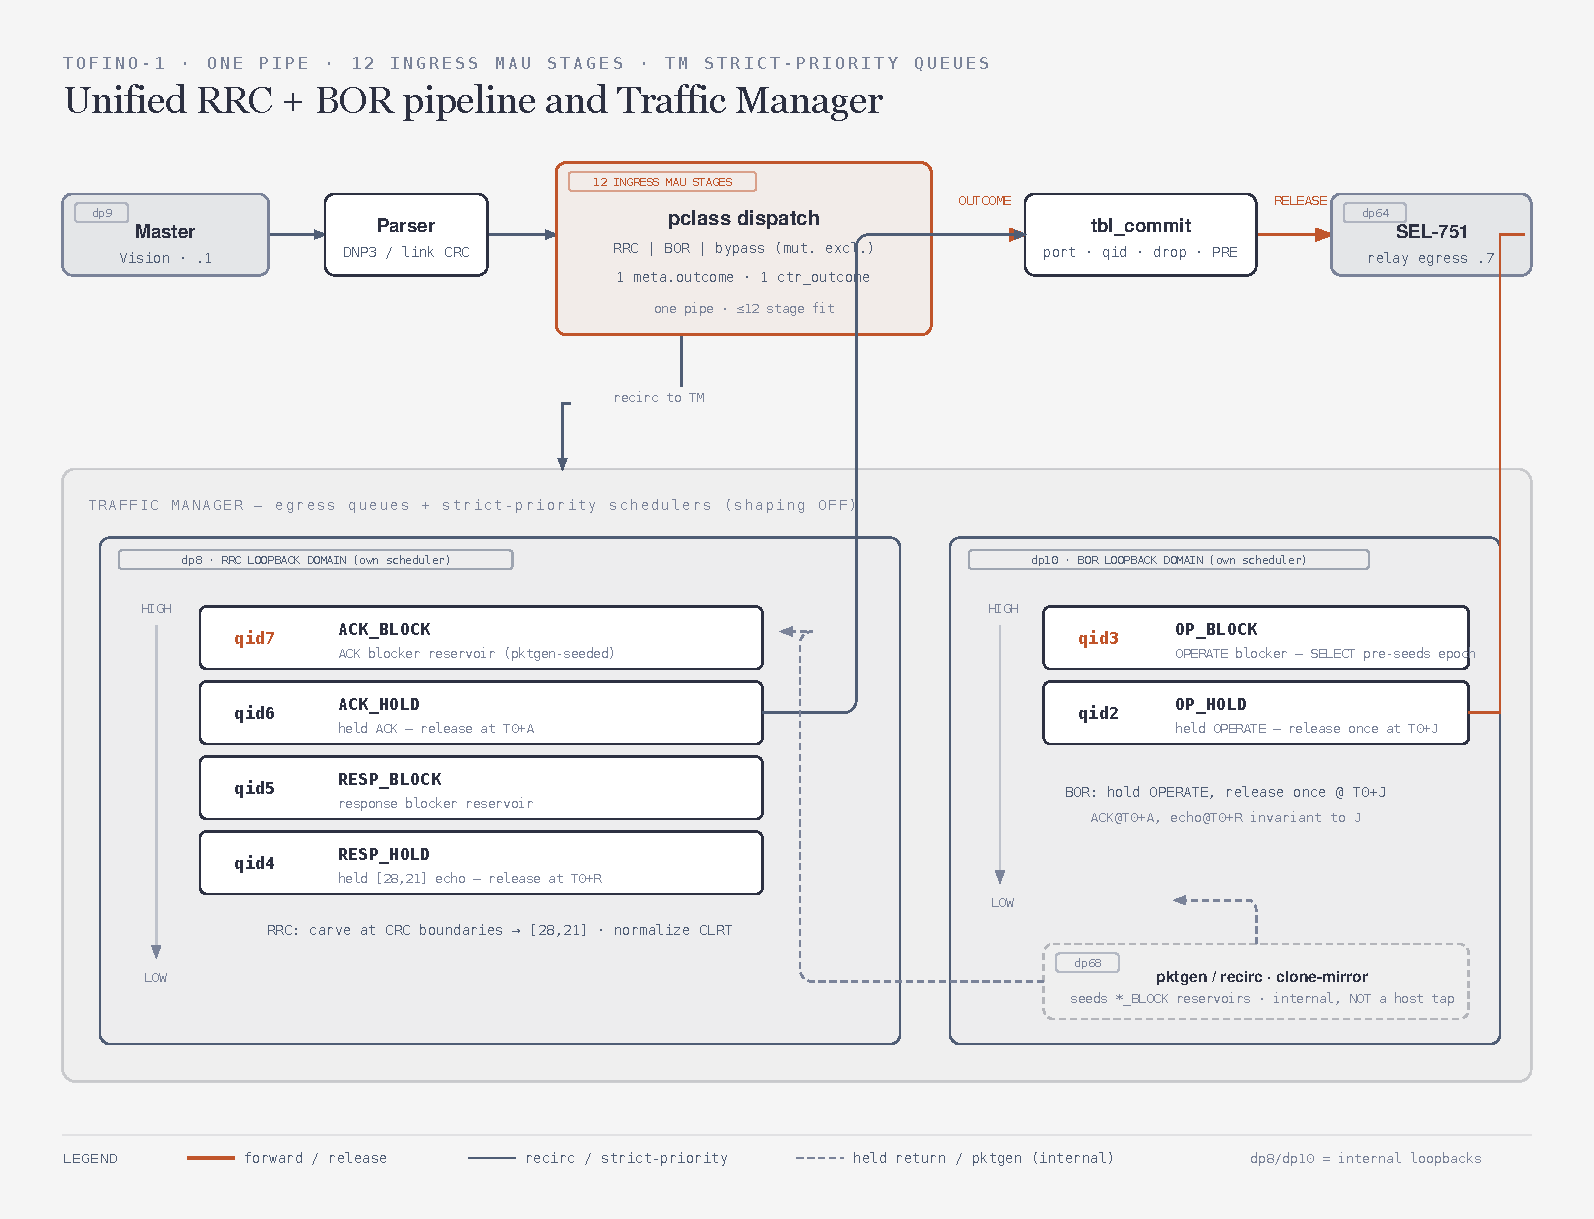
\includegraphics[width=0.95\textwidth]{figures/fig_pipeline}
\caption{One-program pipeline and the two scheduling domains. The parser and match-action stages
compute a single \code{meta.outcome} that a terminal \code{tbl\_commit} applies. The Traffic Manager
holds the response-shaping reservoirs on \code{dp8} (queues \code{qid7}--\code{qid4}) and the control-command queue pair on
\code{dp10} (\code{qid3},\code{qid2}); the packet generator on \code{dp68} seeds the blocker
reservoirs. Egress carves the eligible response to $[28,21]$.}
\label{fig:pipeline}
\end{figure*}

\subsection{One-program pipeline and the single commit}
\textbf{One outcome, one commit.} Figure~\ref{fig:pipeline} shows the pipeline. Earlier match-action
logic computes a compact result
\code{meta.outcome}; a terminal table \code{tbl\_commit} keyed on that result applies the port, queue,
drop, bypass, or multicast effect and is the only stage that writes those fields. The map is
constant and total over every defined outcome, and its default action forwards the packet unmodified
rather than dropping it, so a program loaded before the control plane runs still forwards traffic.
This structure keeps the disposition auditable from a single table and is what lets the two mechanisms share
one ingress pipe within twelve stages: a decision-table flatten collapses the branch tree into two
mutually exclusive ternary tables that co-place in one stage and feed the single commit.

\subsection{Parser and transaction classification}
The parser recognizes Ethernet, IPv4, TCP, and the DNP3 link, transport, and application headers, and
rejects IP fragments and non-TCP traffic to the forwarding default. Classification folds READ, SELECT,
and OPERATE into one role at parse time and re-derives the DNP3 function code inside the pipeline,
producing a control byte that gates every downstream decision. A returning recirculated packet is
identified by its ingress port and then keyed on its content, not on the port, so the same logic
applies regardless of which internal loopback delivered it. Generated tokens and clones are
recognized by a parser value set and a leading tag byte.

\subsection{Absolute timestamps and deadlines}
\textbf{Anchoring to the request.} On the request or OPERATE, the pipeline records an ingress
timestamp $T_0$ and arms two deadlines, $T_0{+}A$ for the ACK and $T_0{+}R$ for the response, from the
policy offsets $A$ and $R$. Anchoring to $T_0$ rather than to the relay's later ACK is required for
the control-command timing argument: because the ACK exists only after the held OPERATE is released, an
ACK-relative deadline would expose the hidden hold. The later relay ACK cannot re-anchor a deadline
once $T_0$ has set it. The offline model verifies this anchoring against a mutant that arms the
deadline at the ACK, which the invariant kills.

\subsection{Packet generation and blocker reservoirs}
\textbf{Reservoirs as timing gates.} A held ACK or response sits in its queue behind a higher-priority
reservoir of generated blocker packets; strict priority drains the blockers first, so the held packet
cannot leave until its reservoir empties at the policy deadline. The on-chip packet generator on
\code{dp68} fills these reservoirs; it never generates master or relay traffic. Two generator profiles
are pinned to distinct tag bytes so that a READ or SELECT arm and an OPERATE hold trigger different
reservoir sets without ambiguity, a separation that a single shared tag did not provide. The reservoir
depth is fixed at $K{=}64$.

\subsection{Response shaping: release, replication, and carving}
Response shaping normalizes the segment shape and the ACK-to-response timing of an
eligible 49-byte response in four steps. \emph{First}, the strict-priority reservoirs hold the real
ACK and the real response on the \code{dp8} ladder across queues \code{qid7} (ACK blocker),
\code{qid6} (ACK hold), \code{qid5} (response blocker), and \code{qid4} (response hold).
\emph{Second}, the ACK and the response release at the absolute offsets $T_0{+}A$ and $T_0{+}R$, so the
master-visible cross-layer response time $\mathrm{CLRT}=R-A$ is a fixed policy value. \emph{Third}, the
release event steers the eligible response into a Packet-Replication-Engine multicast group, which
produces two master-facing copies. \emph{Last}, egress carving emits the 28-byte prefix from one copy
and the 21-byte suffix from the other, advancing the suffix TCP sequence number by 28 so the two
segments abut. The physical relay produces the response; PRE replication produces the two copies used
for segmentation, and no clone or mirror fabricates the response. No DNP3 byte is modified and no DNP3
CRC is recomputed; only the IPv4 and TCP checksums are recomputed over each emitted window. Byte~28 is
a selected existing DNP3 CRC-block boundary that simplifies deterministic carving and validation; TCP
may segment a byte stream at any offset, so this is a design choice, not a protocol requirement, and
the reassembled response remains 49 bytes. Figure~\ref{fig:carve} shows the 49-byte response and the
carve: the prefix is the 10-byte link header plus the first CRC-protected data block, and the suffix
is the remaining blocks, so each emitted segment ends on an already-valid CRC.

\begin{figure}[t]
\centering
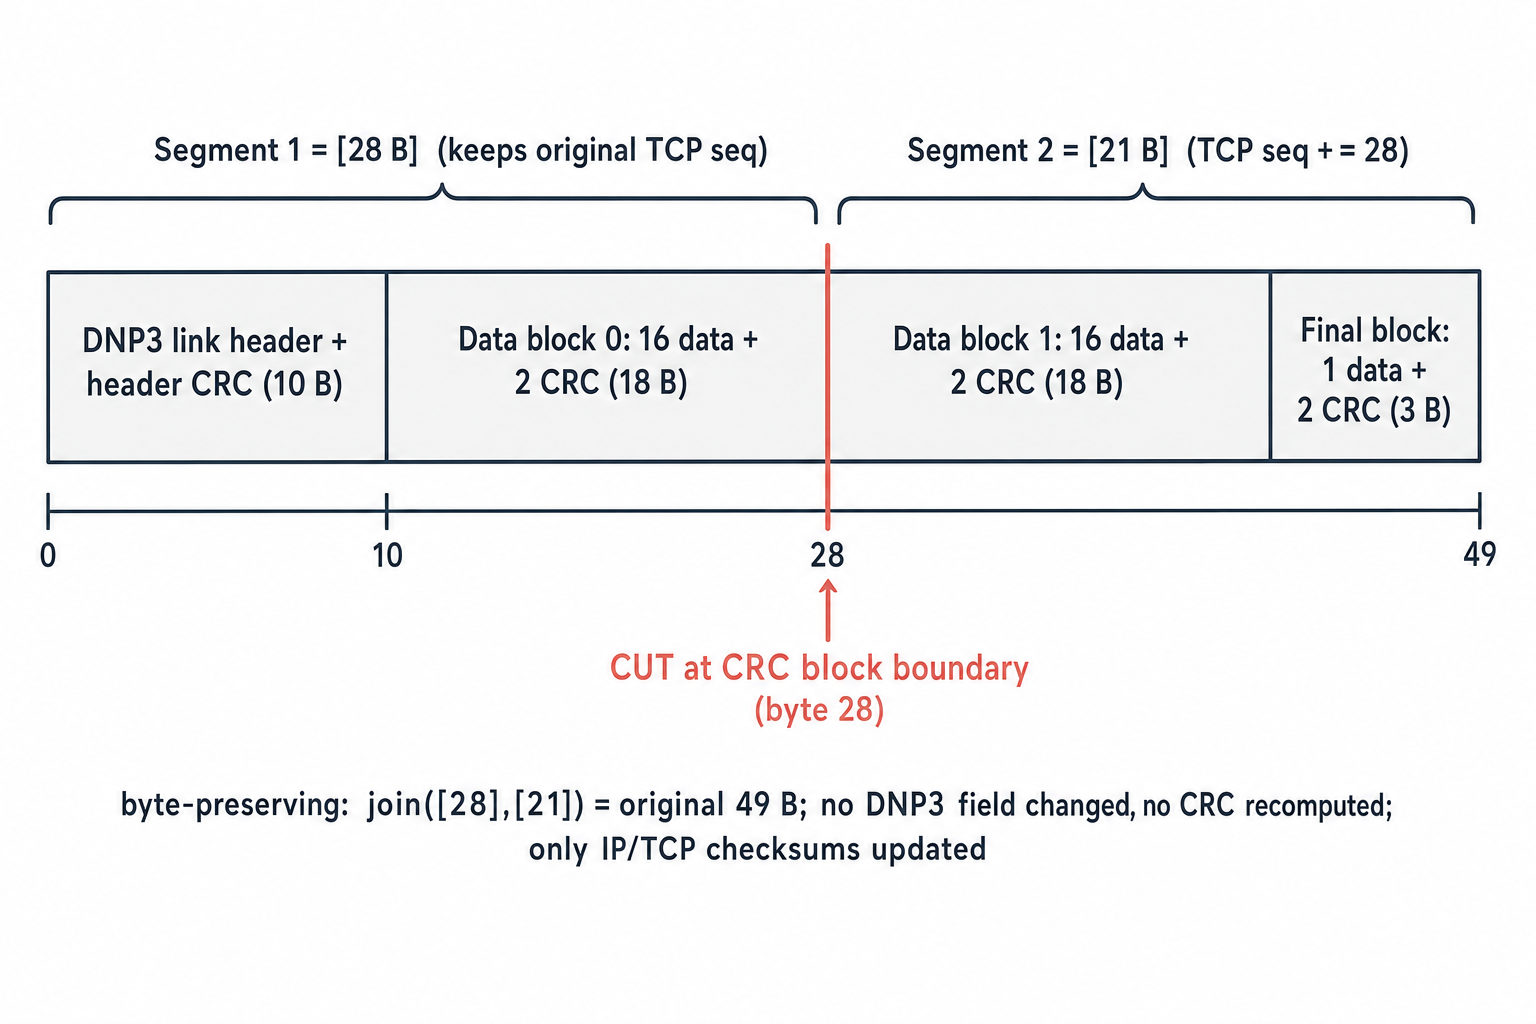
\includegraphics[width=0.98\columnwidth]{figures/fig_carve}
\caption{The 49-byte SEL-751 response and the $[28,21]$ carve. The cut at byte~28 falls on an existing
DNP3 CRC-block boundary; the prefix keeps the original TCP sequence number and the suffix advances it
by 28, so the master reassembles the identical 49-byte response. No DNP3 byte is modified and no CRC is
recomputed.}
\label{fig:carve}
\end{figure}

\subsection{Control commands: block the OPERATE, then release it once}
The control-command hold governs the one control command. \textbf{Preparing an epoch.} A
SELECT crossing the pipeline pre-seeds the OPERATE blocker reservoir on \code{dp10}, so the hold is
armed before the OPERATE arrives; the epoch is an internal per-transaction marker, not the DNP3
sequence. \textbf{Holding and releasing.} The switch admits one matching OPERATE, holds it in
\code{qid2} behind the \code{qid3} reservoir, and is designed to release it once at $T_0{+}J$, where
$J$ is drawn in the data plane from a bounded codebook so that a passive observer cannot predict it
from public header fields. \textbf{Master-visible placement.} The ACK and echo release to the master
at $T_0{+}A$ and $T_0{+}R$, anchored to the original $T_0$ and independent of $J$, so the observable
gap $\mathrm{echo}-\mathrm{ACK}=R-A$ carries no information about the hold. \textbf{Retirement.} After
release the generation is kept as a spent marker until the next SELECT; a retransmitted OPERATE that
reads the spent marker is classified a duplicate and dropped. The hardware captures establish the
master-visible placement and the invariant gap; the offline model verifies the release-at-$T_0{+}J$
state machine; the relay-facing $T_0{+}J$ timestamp and delivery multiplicity are not directly
observed, because \code{dp68} is internal and no relay-facing tap was captured.

\subsection{Two independent scheduling domains}
\textbf{Why two domains.} Response shaping seeds ACK and response reservoirs on high-priority queues. On one shared
strict-priority ladder those reservoirs starve the OPERATE blocker and hold queues after the OPERATE
arrives, which shifts the release toward $A$ or $R$ instead of $T_0{+}J$. The final design places the
response-shaping ladder on \code{dp8} and the control-command queue pair on \code{dp10}, so each mechanism arbitrates on its own
egress scheduler. Both loopbacks are internal paths in the same physical Tofino and the same P4
program; the separation removes the coupling without adding an inline device or a second pipe.

\subsection{Control plane and readback}
The control-plane layer brings up the ports, creates the Traffic-Manager queues at descending
strict-priority levels with shaping disabled, installs the multicast group and mirror session, writes
the session and timing parameters and the $J$ codebook, and initializes the control-command registers. Every write
is read back and compared, and a mismatch or a configuration warning leaves the mechanism disabled
rather than partially configured. There is no configuration snapshot; rollback is a forward,
readback-checked teardown to a plain forwarding state.

\subsection{Failure behavior}
\textbf{Fail open.} On a missing state, an unarmed deadline, or an unrecognized class, the terminal
commit forwards the packet unmodified; the design never drops on the default path. A retransmitted
OPERATE after release is dropped as a duplicate rather than re-forwarded. Traffic outside the eligible
49-byte class, unsupported DNP3 functions, and malformed frames bypass shaping and forward natively.
The control-command timing argument holds only on a flow without TCP timestamps; the pipeline gates on the
timestamp option and the evaluated captures carry none.

\subsection{Safety guard and testbed restoration}
The control-test harness that issues a physical SELECT and OPERATE is guarded: it permits only the
isolated CROB points \code{\{1,3\}} and refuses the breaker-close index~6. Across every guarded
transaction, all 32 relay outputs remained OPEN, and no breaker operation was attempted. Native and
defended trials use the same master, SEL-751, links, switch, capture clock, and loaded binary,
separated only by a runtime mode change, so the comparison isolates the defense rather than the
environment.

\subsection{Resource fit and implementation limitations}
The program compiles for one Tofino-1 ingress pipe within the twelve-stage budget; the control-command state uses
four registers in a domain gated so that an OPERATE token never reaches the response-shaping registers. The
implementation does not observe the relay-facing link, does not normalize the total reassembled
response length, and is evaluated on one outstation; Section~\ref{sec:eval} reports the measured
consequences of these bounds. \textbf{Repeatability.} The loaded source and binary are identified by
hash, the analysis regenerates deterministically from the captured traces, and a manifest verifies
every derived artifact.
